\documentclass[ngerman, aspectratio=169]{beamer}

%style
\mode<presentation>{
	\usetheme{Frankfurt}
}
%packages
\usepackage[utf8]{inputenc}
\usepackage[english]{babel}
\usepackage{graphicx}
\usepackage{array}

\newcolumntype{L}[1]{>{\raggedright\let\newline\\\arraybackslash\hspace{0pt}}m{#1}}
\usepackage{ragged2e}

\usepackage{bm} % bold math
\usepackage{amsfonts}
\usepackage{amssymb}
\usepackage{mathtools}
\usepackage{amsmath}
\usepackage{multirow} % multi row in tables
\usepackage{scrextend}

\usepackage{tikz}

\usepackage{algorithmic}

%\usepackage{algorithm} % http://ctan.org/pkg/algorithm
%\usepackage{algpseudocode} % http://ctan.org/pkg/algorithmicx

%\usepackage{algorithmicx}


%citations
\usepackage[style=verbose,backend=biber]{biblatex}
\addbibresource{references.bib}



\usefonttheme[onlymath]{serif}

%Beamer Template modifications
%\definecolor{mainColor}{HTML}{0065A3} % HSR blue
\definecolor{mainColor}{HTML}{D72864} % OST pink
\definecolor{invColor}{HTML}{28d79b} % OST pink
\definecolor{dgreen}{HTML}{38ad36} % Dark green

%\definecolor{mainColor}{HTML}{000000} % HSR blue
\setbeamercolor{palette primary}{bg=white,fg=mainColor}
\setbeamercolor{palette secondary}{bg=orange,fg=mainColor}
\setbeamercolor{palette tertiary}{bg=yellow,fg=red}
\setbeamercolor{palette quaternary}{bg=mainColor,fg=white} %bg = Top bar, fg = active top bar topic
\setbeamercolor{structure}{fg=black} % itemize, enumerate, etc (bullet points)
\setbeamercolor{section in toc}{fg=black} % TOC sections
\setbeamertemplate{section in toc}[sections numbered]
\setbeamertemplate{subsection in toc}{%
	\hspace{1.2em}{$\bullet$}~\inserttocsubsection\par}

\setbeamertemplate{itemize items}[circle]
\setbeamertemplate{description item}[circle]
\setbeamertemplate{title page}[default][colsep=-4bp,rounded=true]
\beamertemplatenavigationsymbolsempty

\setbeamercolor{footline}{fg=gray}
\setbeamertemplate{footline}{%
	\hfill\usebeamertemplate***{navigation symbols}
	\hspace{0.5cm}
	\insertframenumber{}\hspace{0.2cm}\vspace{0.2cm}
}

\usepackage{caption}
\captionsetup{labelformat=empty}

%Title Page
\title{Der Satz von Poincaré-Bendixson}
\author{Raphael Unterer}
\institute{Mathematisches Seminar 2025: Felder}

\newcommand*{\HL}{\textcolor{mainColor}}
\newcommand*{\RD}{\textcolor{red}}
\newcommand*{\BL}{\textcolor{blue}}
\newcommand*{\GN}{\textcolor{dgreen}}
\newcommand*{\YE}{\textcolor{violet}}




\makeatletter
\newcount\my@repeat@count
\newcommand{\myrepeat}[2]{%
	\begingroup
	\my@repeat@count=\z@
	\@whilenum\my@repeat@count<#1\do{#2\advance\my@repeat@count\@ne}%
	\endgroup
}
\makeatother




\usetikzlibrary{automata,arrows,positioning,calc}


\begin{document}

	%Titelseite
	\begin{frame}
		\titlepage
	\end{frame}

	\section{Motivation}
    \begin{frame}
        \frametitle{El Niño Southern Oscillation (ENSO)}
        \begin{center}
            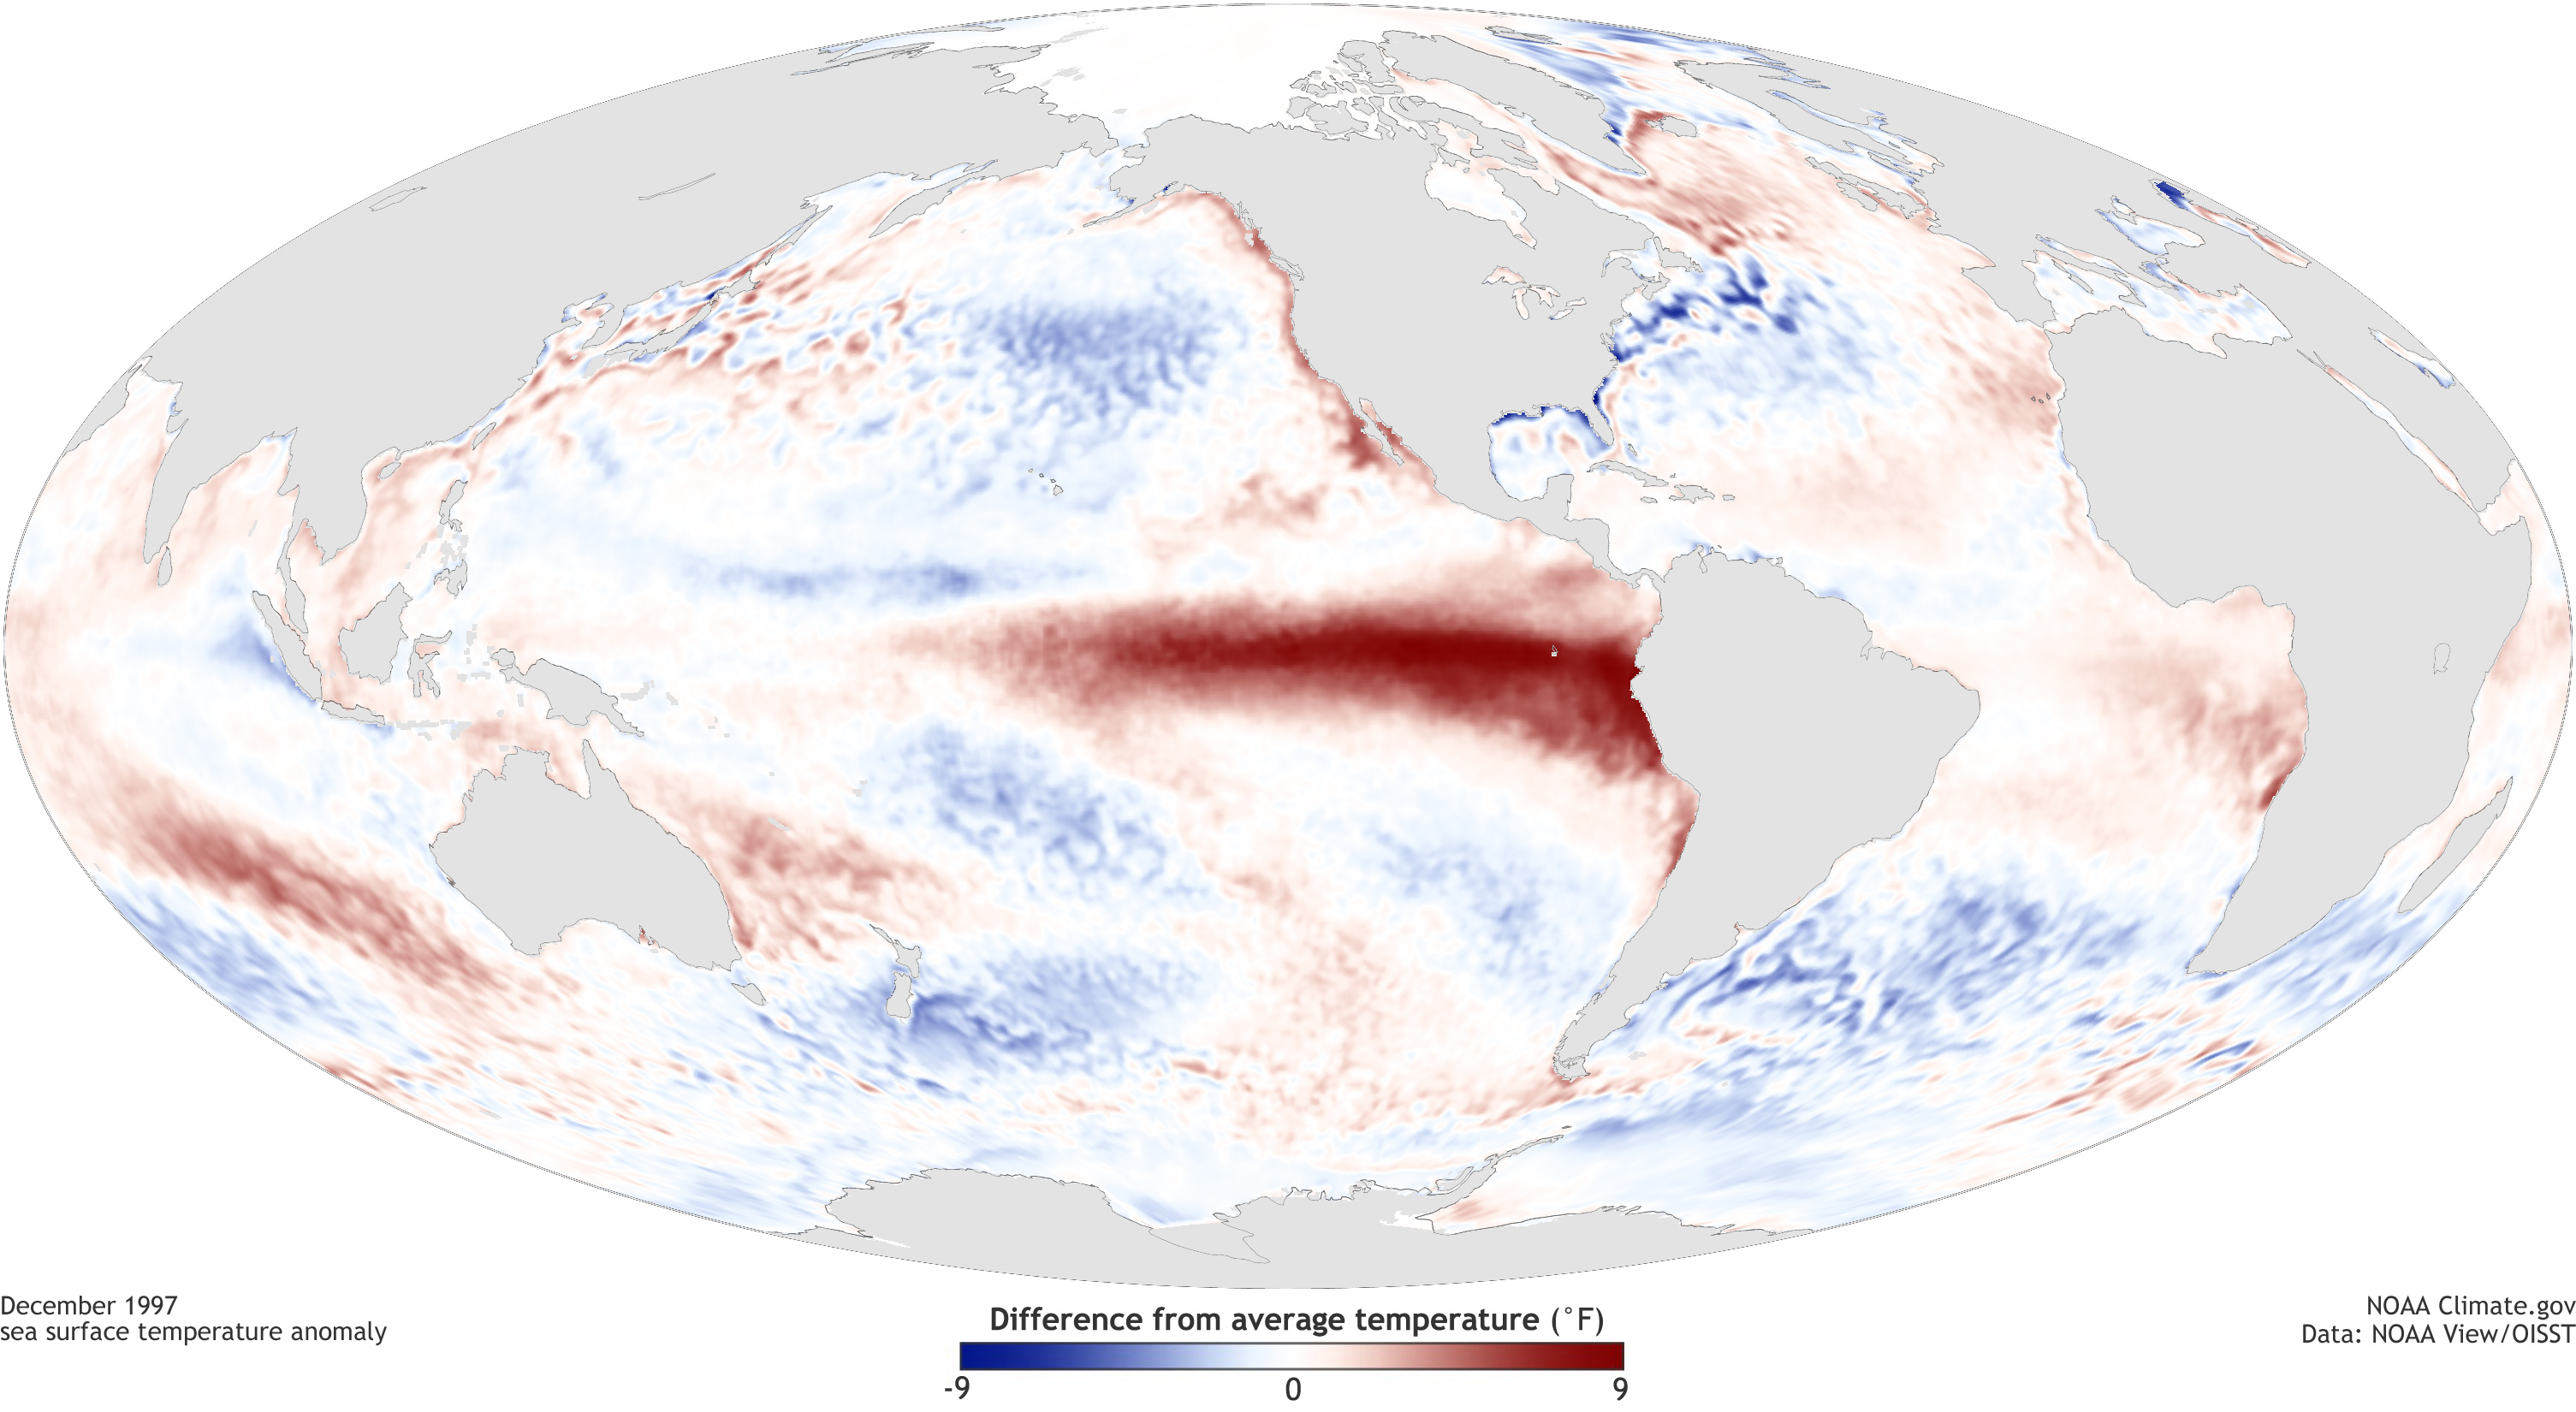
\includegraphics[width=0.7\textwidth]{../images/iconic_ENSO_elNino_lrg.jpg}
        \end{center}
    \end{frame}

    \begin{frame}
        \frametitle{El Niño Southern Oscillation (ENSO)}
        \begin{center}
            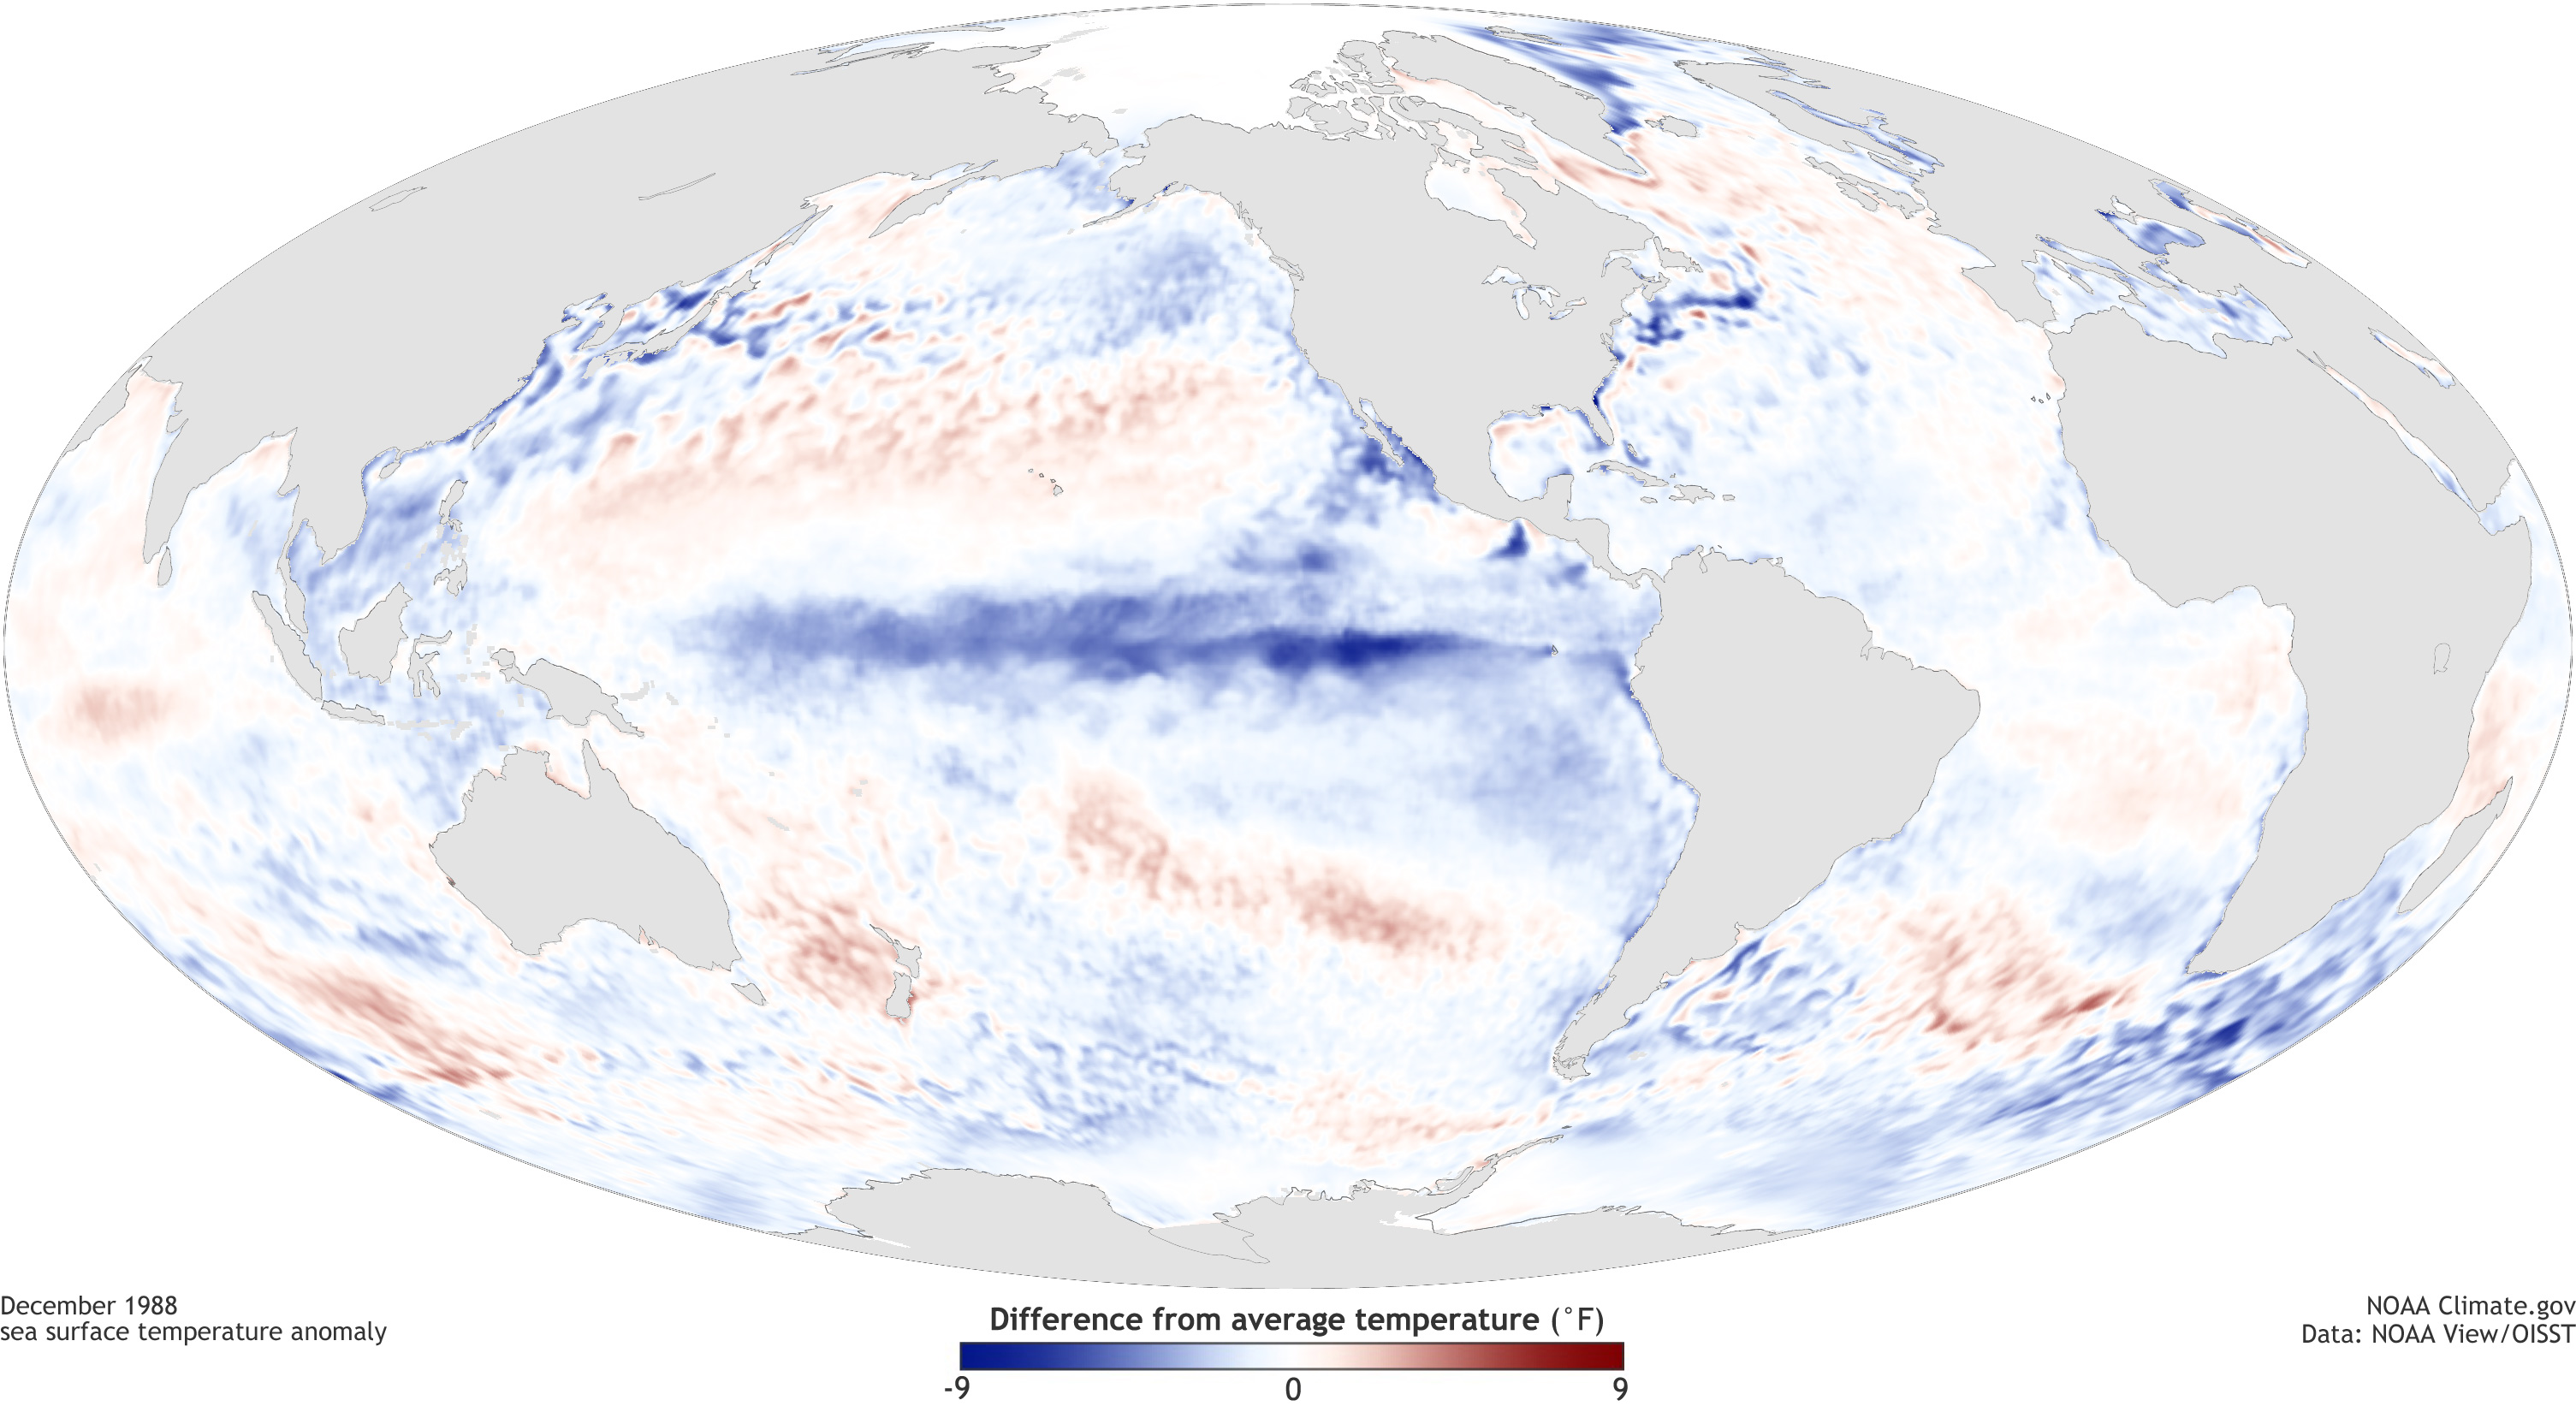
\includegraphics[width=0.7\textwidth]{../images/iconic_ENSO_laNina_lrg.jpg}
        \end{center}
    \end{frame}

    \begin{frame}
        \frametitle{El Niño Southern Oscillation (ENSO)}
        \begin{center}
            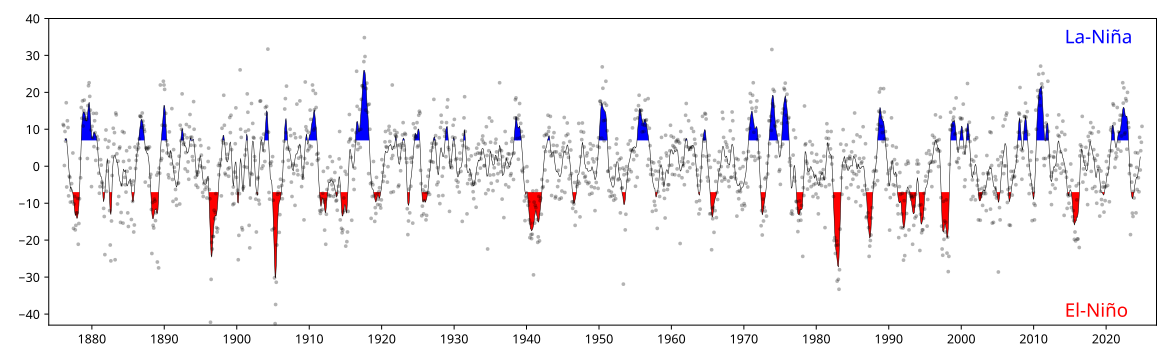
\includegraphics[width=\textwidth]{../images/elnino_data.png}
        \end{center}
    \end{frame}

    \begin{frame}
        \frametitle{Modellierung als dynamisches System}
        Recharge Oscillator Modell:
        \begin{align*}
            \frac{dT_e}{dt} &= -cT_e + \gamma \left(bT_E + h_W\right) - \epsilon \left(bT_E + h_W\right)^3, \\
            \frac{dh_W}{dt} &= -rh_W - \alpha b T_E.
        \end{align*}
        \pause
        Vereinfachen:
        \begin{align*}
            \dot{x} &= -x + \gamma \left(bx + y\right) - \epsilon \left(bx + y\right)^3, \\
            \dot{y} &= -ry - \alpha b x.
        \end{align*}
    \end{frame}

    \begin{frame}
    \frametitle{Gewünschte Eigenschaften}
        Das Recharge Oscillator ENSO Modell soll folgende Eigenschaften haben:
        \begin{itemize}
            \item Oszillierend
            \item Kleine Änderungen der Parameter ändert nicht viel an der Lösung
            \item Anfangsbedingungen spielen keine grosse Rolle
        \end{itemize}
    \end{frame}

	\section{Poincaré-Bendixson}
    \begin{frame}
    \frametitle{Limesmengen}
        Dynamisches System $\Phi_t(p)$ hat die Alpha- und Omega-Limesmenge:

        \begin{align*}
            \alpha(p) &= \lim_{t\to-\infty} \Phi_t(p) = Y \\
            \omega(p) &= \lim_{t\to\infty} \Phi_t(p) = Y
        \end{align*}
    \end{frame}
    \begin{frame}
    \frametitle{Voraussetzungen für Poincaré-Bendixson}
        \begin{itemize}
            \item Dynamisches System $\Phi_t(p) \in \Xi^r(\mathbb{R}^2)$
            \item Finite Anzahl Singularitäten
            \item Anfangspunkt $p \in \mathbb{R}^2$
        \end{itemize}
    \end{frame}
    \begin{frame}
    \frametitle{Poincaré-Bendixson: Fall 1}
        \begin{enumerate}
            \item $\omega(p)$ ist eine Singularität
        \end{enumerate}
        %TODO Plot
    \end{frame}
    \begin{frame}
    \frametitle{Poincaré-Bendixson: Fall 2}
        \begin{enumerate}
            \setcounter{enumi}{1}
            \item $\omega(p)$ ist ein geschlossener Orbit
        \end{enumerate}
        %TODO Plot
    \end{frame}
    \begin{frame}
    \frametitle{Poincaré-Bendixson: Spezialfall 3}
        \begin{enumerate}
            \setcounter{enumi}{2}
            \item $\omega(p)$ ist ein geschlossener Orbit welcher Singularitäten verbindet
        \end{enumerate}
        %TODO Plot
    \end{frame}
    %Idee: 2D schränkt mögliche Lösungen stark ein. Das kann formuliert werden mit Poinbendix.
    % Wir brauchen dass, da unser ENSO model sehr stark vereinfacht ist.

    \section{Anwendung und Relevanz}
    % Plots von ENSO. Lösungen konvergieren.
    % Idee: Plot wo unterwegs die Gleichung (Konstanten) ändert -> bleibt trotzdem auf einem ähnlichen Orbit
    % Link zum Sonnensystem herstellen!
    % Chaos in 3D möglich: Zeigen des Videos von Müller

\end{document}

